\documentclass[titlepage]{article}
\usepackage[a4paper,includehead,includefoot,headheight=10pt,headsep=2mm,width=17cm,height=27cm,footskip=0.5cm]{geometry}
\usepackage{cmap}
\usepackage{hyperref}
\usepackage[T2A]{fontenc}
\usepackage[utf8]{inputenc}
\usepackage[russian]{babel}
\usepackage{graphicx}
\usepackage{xcolor}
\usepackage{amssymb}
\usepackage{amsmath}
\usepackage{physics}

\usepackage{amsmath}
\DeclareMathOperator\arctanh{arctanh}

\usepackage{amsmath}
\DeclareMathOperator\arccosh{arccosh}

\begin{document}
\begin{flushright}
    Расчётно Графическая Работа №6
    
    Выполнил: Козлов Александр
\end{flushright}

\section{Формулировка задания}

Исследовать при $\beta \longrightarrow 0$ и при $\mu \longrightarrow 0$ стационарные решения (солитоны и ударные волны) уравнения:
\begin{equation}
    \partial_t v + v^3 \partial_x v + \beta \partial_{xxx} v = \mu \partial_{xx} v
\end{equation}

\section{Фазовый портрет}
Первым делом проведём следующие необходимые процедуры.
\begin{enumerate}
 \item Подставляем в уравнение решение в виде стационарной волны: $v = v\qty(\xi)$, где $\xi = x - Vt$. Полагаем $V > 0$. Такая  подстановка приводит к уравнению:
 \begin{equation}
  -Vv' + v^3v' + \beta v''' = \mu v''
 \end{equation}
Полагаем, что решение обращается в нуль на бесконечности. Тогда интегрирование уравнения даёт:
\begin{equation}\label{three}
  -Vv + \dfrac{v^4}{4} + \beta v'' = \mu v'
\end{equation}
\item \label{bla} Исследуем уравнение на фазовой плоскости. Делаем замену и получаем систему уравнений первого порядка.
$$
\begin{cases}
    v'= u \\
    u'= \dfrac{\mu}{\beta}u + \dfrac{V}{\beta}v - \dfrac1{4\beta} v^4
\end{cases}
$$
Данная система имеет две стационарные точки при $u = 0$ и $v = 0,$ $\sqrt[3]{4V}$. На плоскости $\qty(\mu,\beta)$ можно следующим образом изобразить зависимость типа состояния равновесия от параметров задачи.
\begin{figure}[h]
 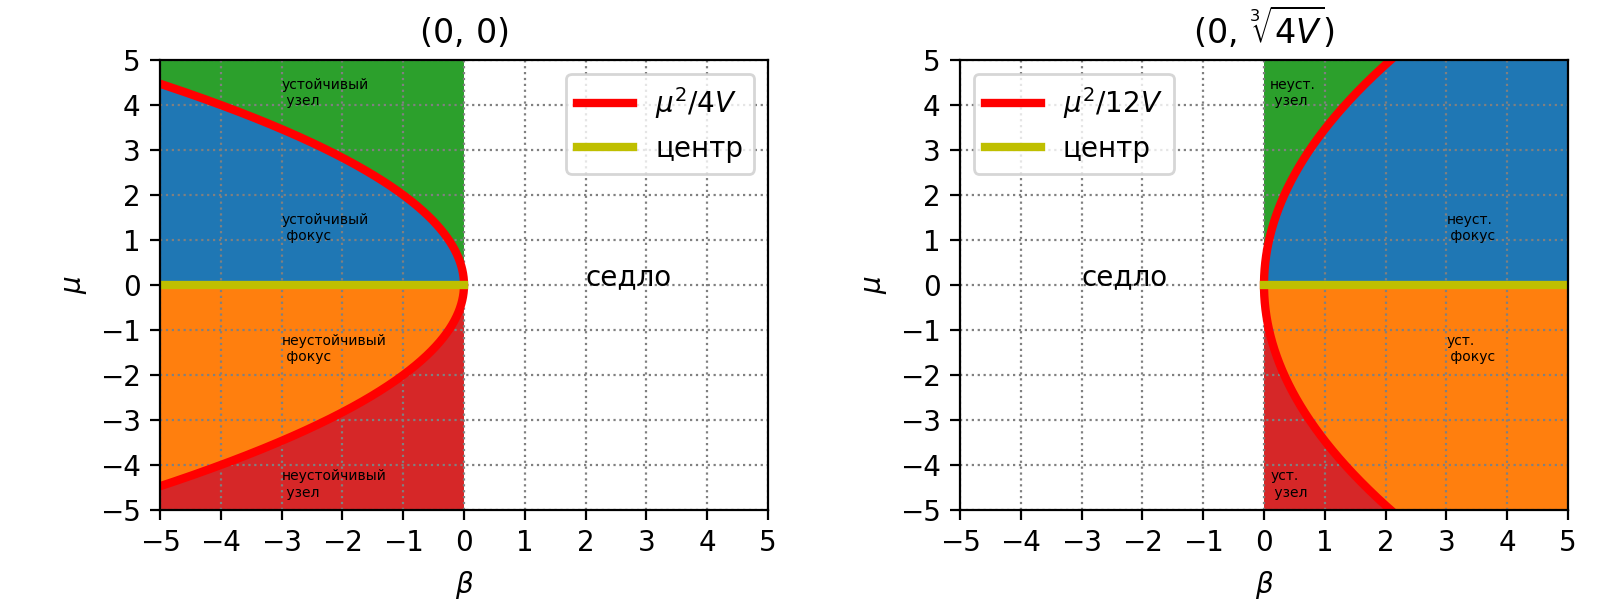
\includegraphics[width = 170 mm]{00.png}
 \caption{Зависимость типа состояния равновесия от параметров задачи}
\end{figure}
\par
Таким образом, становится ясно, что имеется ввиду, когда говорится о $\beta \longrightarrow 0$ и о $\mu \longrightarrow 0$. Нужно сравнивать $\beta$ с $\frac{\mu^2}{4V}$ или с $\frac{\mu^2}{12V}$.
\end{enumerate}

\section{Предельные случаи}
Рассмотрим предельные случаи \--- просто приравняем $\beta$ и $\mu$ к нулю поочерёдно.
\subsection{${\mu = 0}$}
Типы точек равновесия зависят от знака $\beta$, как видно из вышеприведённых картинок. Посему рассмотрение данного предельного случая распадается на двое. В обоих случаях нет диссипации и, следовательно, стационарное решение будет иметь солитонный вид. 
\par Ясно, что диссипация уходит из уравнения в рассматриваемом пределе, что позволяет выделить гамильтониан. Далее, приравняв его значению решения на сепаратрисе (которая соответсвует солитону), понижаем порядок уравнения до перового, что позволяет его просто проинтегрировать. То есть вся сложность уравнения сводится ко взятию интеграла.

\subparagraph{$\beta > 0$}
\begin{enumerate}
 \item Построим фазовую плоскость данного случая.
\begin{figure}[h]
 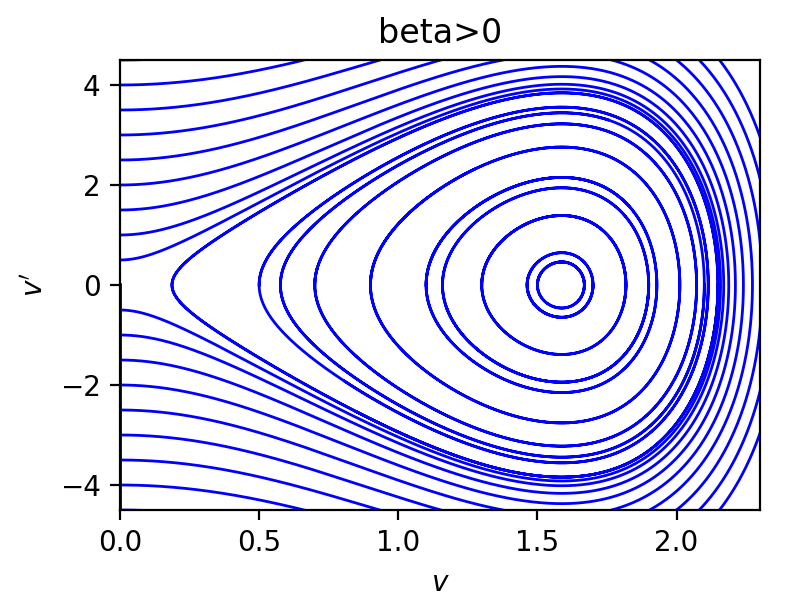
\includegraphics[width = 160 mm]{0-.png}
 \caption{Фазовая плоскость уравнения (\ref{three}) при $\mu=0$ и $\beta=0.1$}
\end{figure}

\item Гамильтониан задачи имеет вид:
\begin{equation}
 H = \frac{\qty(v')^2}{2} - \frac{V v^2}{2\beta} + \frac{v^5}{20\beta} 
\end{equation}
Солитонному решению соответствует нулевой уровень энергии. Получаем интегральное соотношение:
\begin{equation}
 \int \dfrac{\dd{v}}{v\sqrt{\frac{V}{\beta} - \frac{1}{10\beta} v^3}} = \int \dd{\xi}
\end{equation}
Вытаскиваем общий множитель из под корня:
\begin{equation}
 \int \dfrac{\dd{v}}{v\sqrt{1 - \frac{v^3}{10V}}} = \int \sqrt{\frac{V}{\beta}} \dd{\xi}
\end{equation}
И обезразмериваем:
\begin{equation}
 \int  \dfrac{\dd{\zeta}}{\zeta\sqrt{1 - \zeta^3}} = \int \sqrt{\frac{V}{\beta}} \dd{\xi}
\end{equation}
Тогда интегрирование даёт:
\begin{equation}
 -\dfrac23 \arctan{\sqrt{1-\zeta^3}} = \sqrt{\frac{V}{\beta}} \xi
\end{equation}
Производим возвращение к исходным переменным:
\begin{equation}
 -\dfrac23 \arctanh{\sqrt{1-\frac{v^3}{10V}}} = \sqrt{\frac{V}{\beta}} \xi
\end{equation}
Теперь выражаем $v\qty(\xi)$:
\begin{equation}\label{soliton}
 v\qty(\xi) = \dfrac{\sqrt[3]{10V}}{\cosh^{\tfrac23}{\qty(\dfrac32\sqrt{\dfrac{V}{\beta}}\xi)}}
\end{equation}
Таким образом, отсюда видно, что <<ширина>> единичного солитона (то бишь характерный масштаб изменения функции) есть ${ l = \tfrac{2}{3}\sqrt{\tfrac{\beta}{V}}}$, а амплитуда изменения функции ${ A = \sqrt[3]{10V}}$. Кусочек солитона изображён на рисунке (\ref{sol}).
\end{enumerate}
\subparagraph{$\beta < 0$}
\begin{enumerate}
 \item Построим фазовую плоскость данного случая.
\begin{figure}[h]
 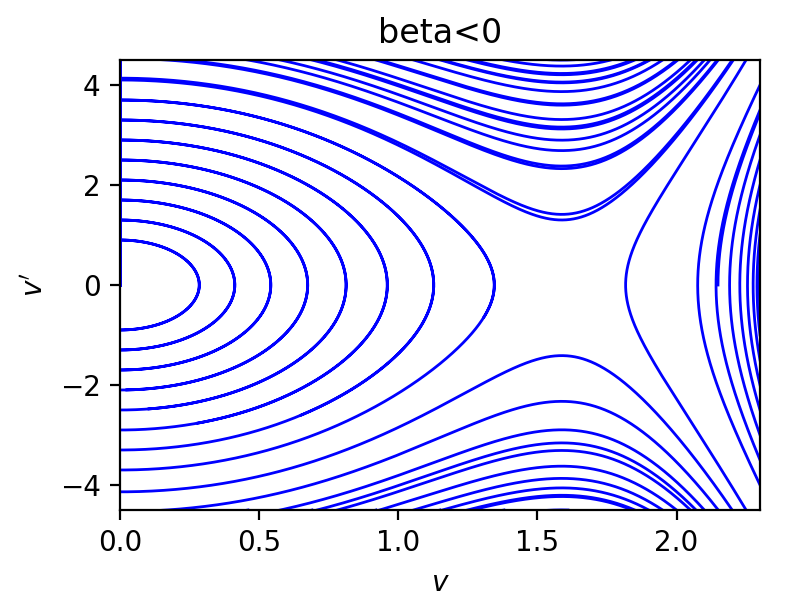
\includegraphics[width = 160 mm]{0+.png}
 \caption{Фазовая плоскость уравнения (\ref{three}) при $\mu=0$ и $\beta=-0.1$}
\end{figure}
\item Гамильтониан задачи имеет вид:
\begin{equation}
 H = \frac{\qty(v')^2}{2} - \frac{V v^2}{2\beta} + \frac{v^5}{20\beta} 
\end{equation}
На сепаратрисе энергия имеет значение $\dfrac{3\,\sqrt[3]{2}}{5}\dfrac{V^{5/3}}{\abs{\beta}}$, тогда интегральное соотношение таково:
\begin{equation}\label{int}
\int \dfrac{\sqrt{\abs{\beta}}\dd{v}}{\sqrt{\frac{6\,\sqrt[3]{2}V^{5/3}}{5}-Vv^2+\frac{v^5}{10}}} = \int \dd{\xi}
\end{equation}
Он не берётся, но можно построить картинку (\ref{pic}). Решение похоже на кинк, как можно видеть.
\begin{figure}[h]
 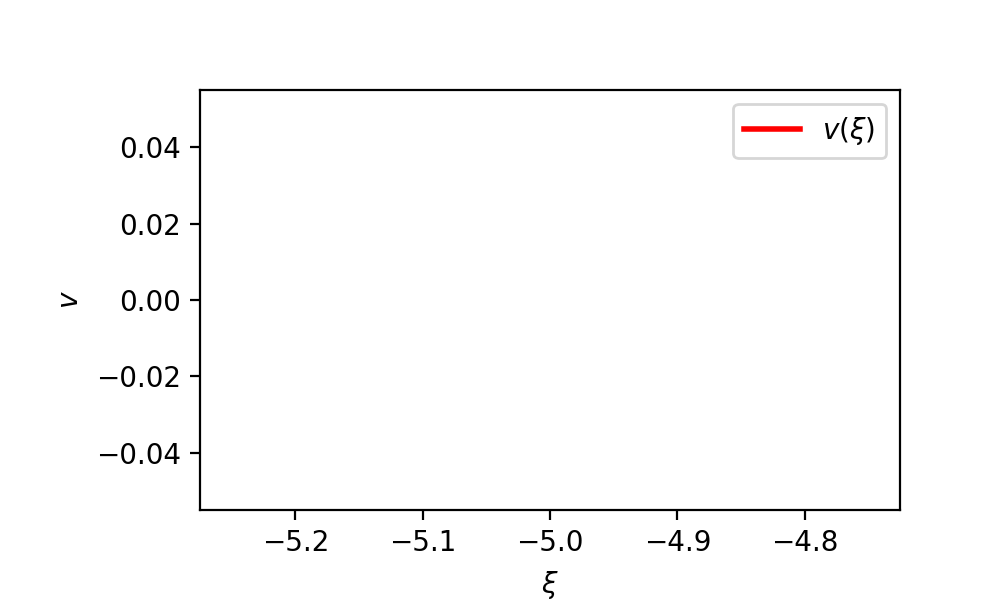
\includegraphics[width = 160 mm]{b0-.png}
 \caption{Численное решение интегрального соотношения (\ref{int}) при $\mu = 0$ и $\beta = -1$}
 \label{pic}
\end{figure}

\end{enumerate}
\subsection{$\beta = 0$}
 В данном случае уравнение (\ref{three}) выглядит:
\begin{equation}
  -Vv + \dfrac{v^4}{4} = \mu v'
\end{equation}
Откуда получается интегральное соотношение:
\begin{equation}
\dfrac1{4\mu} \int \dd{\xi} = \int \dfrac{\dd{v}}{\qty(\dfrac{v^3}{4V} - 1)v}
\end{equation}
Делаем замену $\dfrac{v}{\sqrt[3]{4V}} = \zeta$:
\begin{equation}
\dfrac1{4\mu} \int \dd{\xi} = \int \dfrac{\dd{\zeta}}{\qty(\zeta^3 - 1)\zeta}
\end{equation}
Интегрируем выражение и получаем:
\begin{equation}
\dfrac{\xi}{4\mu} = \ln{\sqrt[3]{\dfrac{1}{\zeta^3} - 1}}
\end{equation}
Окончательный ответ выглядит так:
\begin{equation}
v\qty(\xi) = \sqrt[3]{\dfrac{4V}{\exp{\dfrac{3\xi}{4\mu}} + 1}}
\end{equation}
\begin{figure}[h]
 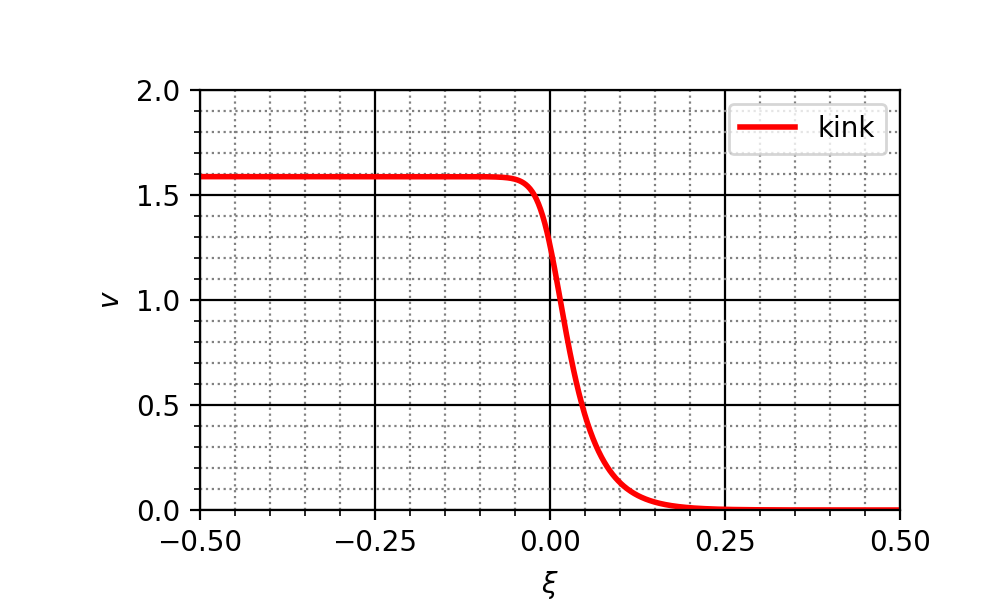
\includegraphics[width = 160 mm]{kink.png}
 \caption{Стационарное решение уравнения (\ref{three}) при $\mu=0.01$ и $\beta=0$}
\end{figure}
\par
Таким образом, в данном случае имеет место ударная волна с шириной фронта $l = \dfrac{4\mu}{3}$ и высотой фронта $A = \sqrt[3]{4V}$.
\section{Многосолитонное решение}
Возможно многосолитонное решение при малых, но отличных от нуля $\mu$, а именно при: 
\begin{equation}
 \abs{\mu} \ll \sqrt{4V\abs{\beta}}
\end{equation}
Получим оценку на расстояние между уединёнными солитонами.Для этого найдем минимальное значение поля $\delta v$ после первого солитона из уравнения на изменение энергии (коэффициенты нужно подбирать аккуратно из сохранения размерности):
\begin{equation}
 \Delta H =  \Delta \qty(- \frac{V \qty(\delta v)^2}{2\beta} + \frac{\qty(\delta v) ^5}{20\beta}) =  - \dfrac{\mu}{\beta} \int \qty(\partial_x v)^2 \dd{\xi}
\end{equation}
Поскольку мы считаем затухание слабым, то в правой части мы можем подставить невозмущенное решение в виде солитона (\ref{soliton}). Минимум решения близок к нулю, посему оставляем только меньшие степени $\delta v$. Тогда получаем:
\begin{equation}
 \qty(\delta v)^2 =  \dfrac{2\mu}{\beta} \int \qty(\sqrt[3]{10V\cosh^{-5}{\qty(\tfrac32\sqrt{\tfrac{V}{\beta}}\xi)}}\sinh{\qty(\tfrac32\sqrt{\tfrac{V}{\beta}}\xi)} )^2 \dd{\xi}
\end{equation}
Обезразмериваем интеграл, вводя новую переменную $\tfrac32\sqrt{\tfrac{V}{\beta}}\xi = \phi$:
\begin{equation}
 \qty(\delta v)^2 =  \dfrac{4\sqrt[3]{10}\mu}{3\sqrt{\beta }\sqrt[6]{V}}  \int \qty(\sqrt[3]{\cosh^{-5}{\qty(\phi)}}\sinh{\phi} )^2 \dd{\phi}
\end{equation}
После взятия интеграла получаем следующий ответ:
\begin{equation}
 \qty(\delta v)^2 = \dfrac{27 719 \sqrt[3]{10}}{18 750} \dfrac{\mu}{\sqrt{\beta }\sqrt[6]{V}}   \varpropto \mu
\end{equation}
Теперь нужно найти решение, соответствующее фазовой траектории, близкой к седлу. То есть полагаем $v \approx 0$ и линериализуем уравнение (\ref{three}):
\begin{equation}
  -Vv + \beta v'' = 0
\end{equation}
Его решением выбираем следующее:
\begin{equation}
 v = \delta v \cosh{\qty(\dfrac23\dfrac{\xi}{l})}
\end{equation}
Сшиваем решение c уединённым солитоном:
\begin{equation}
 \cosh^{\tfrac53}{\qty(\dfrac{L}{l})} = \dfrac{\sqrt[3]{10V}}{\sqrt{\dfrac{27 719 \sqrt[3]{10}}{18 750} \dfrac{\mu}{\sqrt{\beta }\sqrt[6]{V}}}}
\end{equation}
В итоге получается следующая оценка на расстояние между солитонами во многосолитонном решении:
\begin{equation}
 {L} =  \frac{l}{10}\ln{ \qty(\dfrac{281\,250\:V^3\:\:l}{27\,719\: \mu})} 
 \approx \frac{l}{10}\ln{ \qty(\dfrac{10\:V^3\:\:l}{\mu})}
\end{equation}
\begin{figure}[h]
 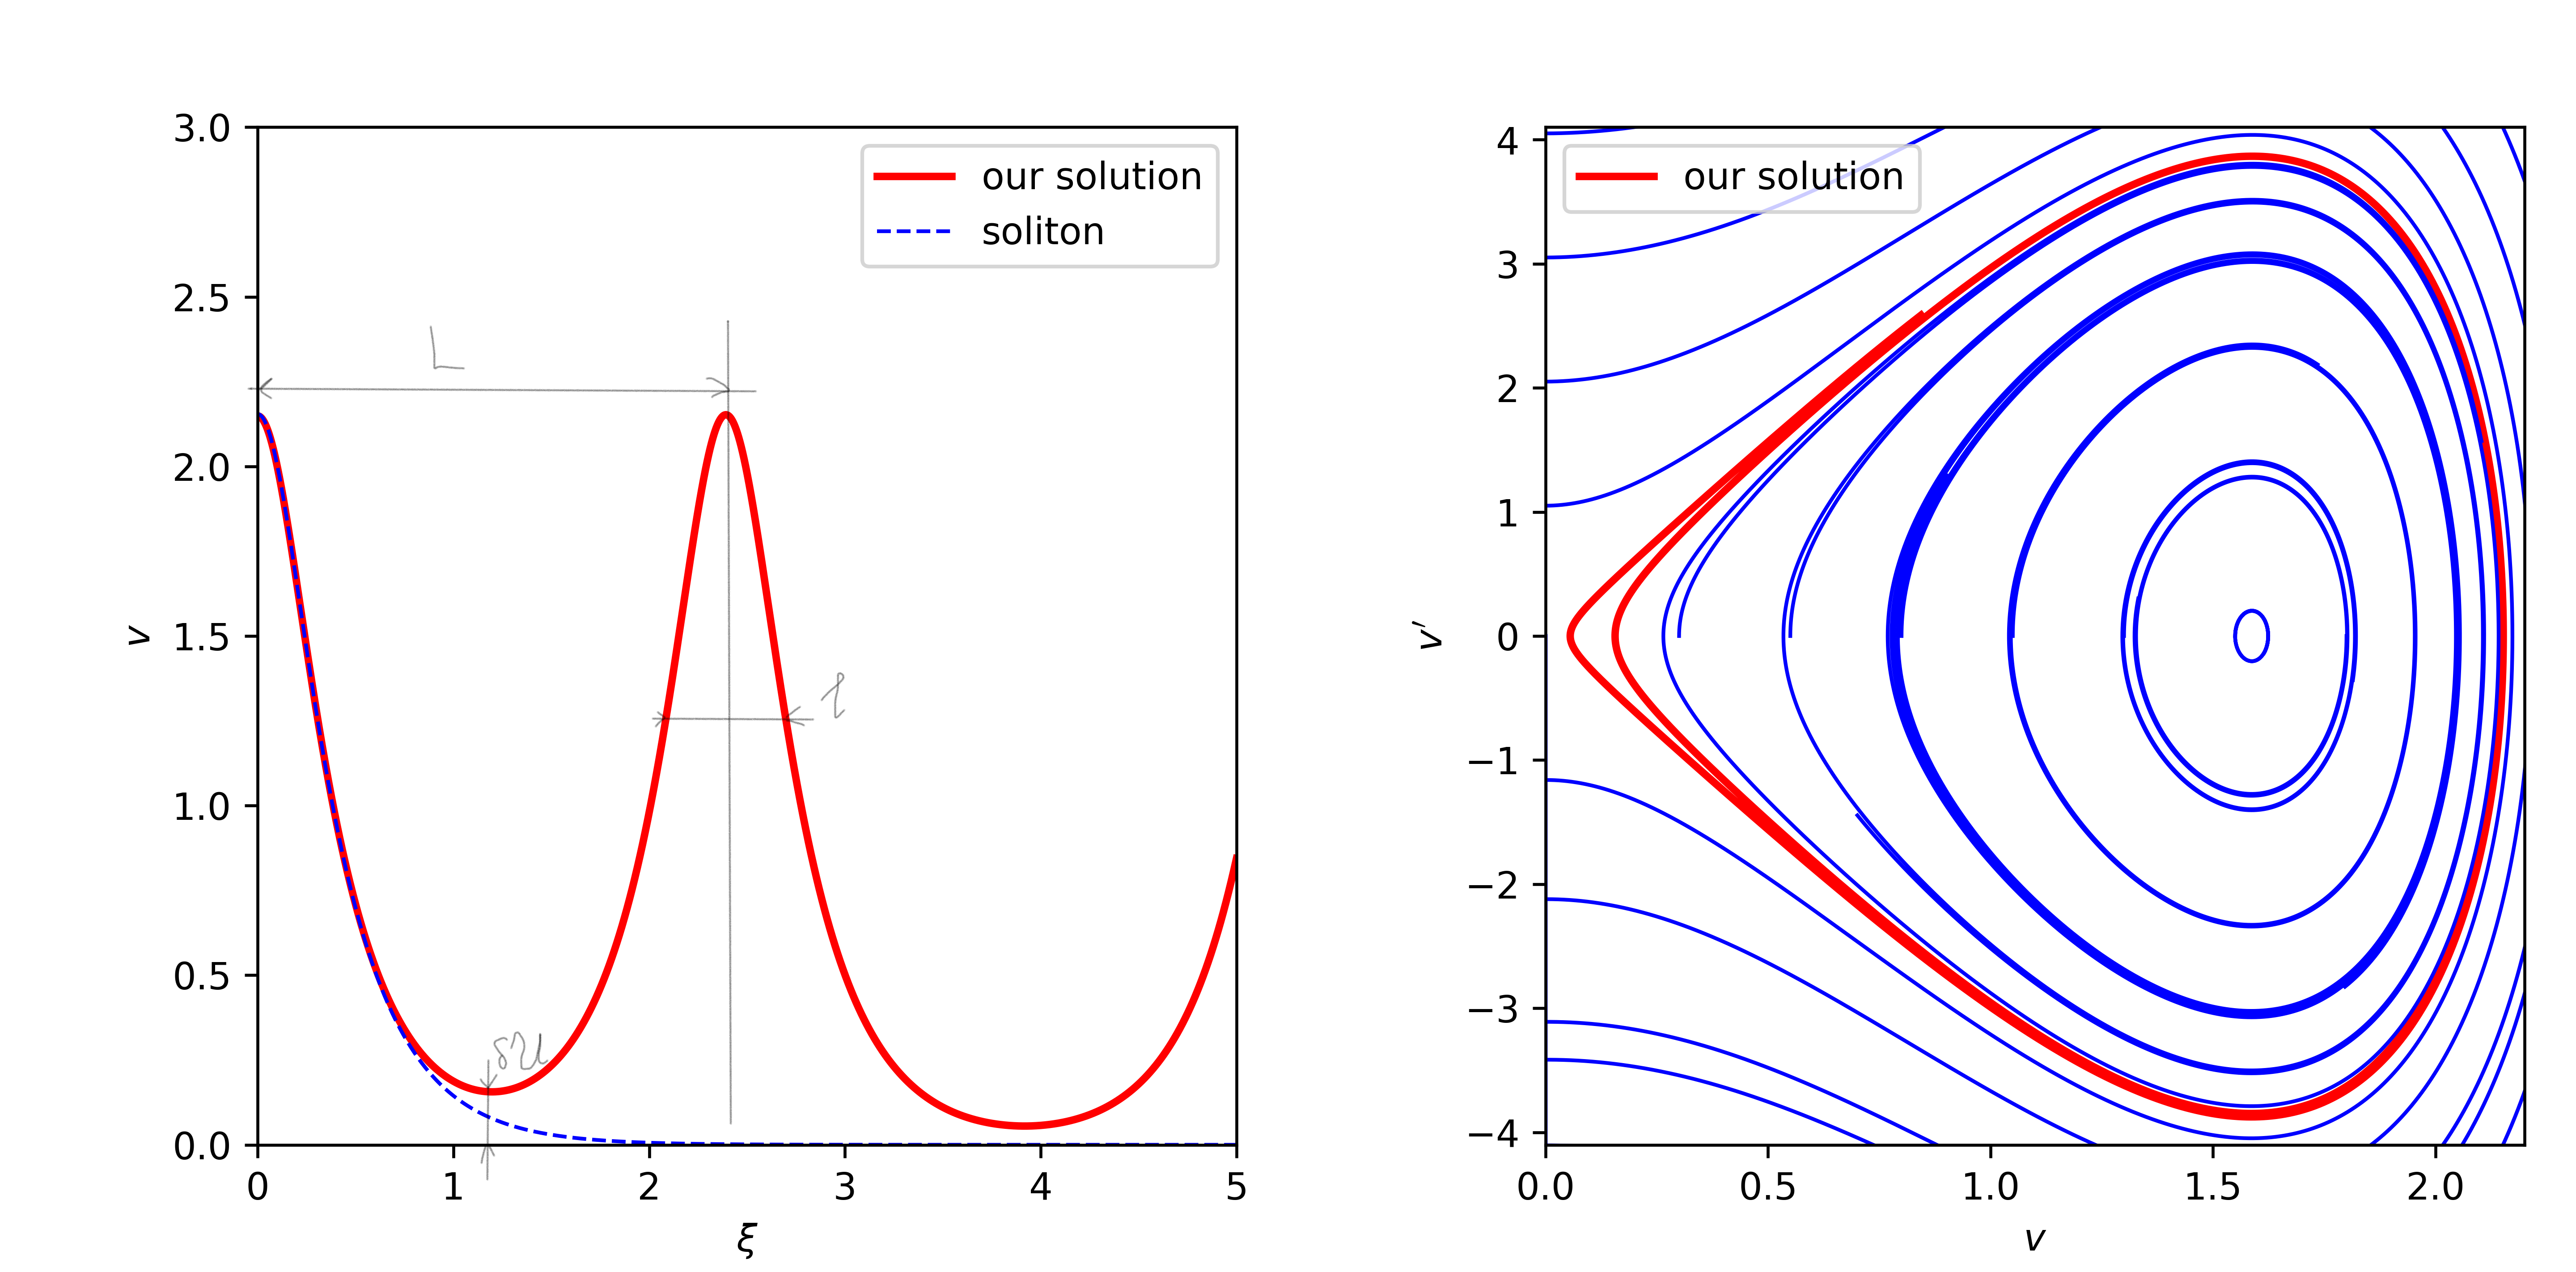
\includegraphics[width = 160 mm]{plo1t.png}
 \caption{На левом графике изображено численное решение уравнения (\ref{three}) с параметрами $\mu = 0.001$, $\beta = 0.1$ и $V = 1$; на правом изображена фазовая плоскость уравнения}
 \label{sol}
\end{figure}
\end{document}
